\section{Incremental Synthesis}
\label{sec:interactive:incremental}

In this section, I present the final enhancement we explored in the context of interactive program synthesis --
\emph{incremental synthesis}.
In conventional synthesis, the learner uses the refined spec $\spec'$ at each iteration to synthesize a new valid
program set $\vsa \models \spec'$.
All the information accumulated in the synthesis session is contained in $\spec'$ as a conjunction of provided examples,
counterexamples, and more general constraints.
Typically in PBE, the learner takes it all into account by solving a fresh synthesis problem, searching in the DSL
$\dsl$ for programs that are consistent with all constraints in $\spec'$.
As the size of $\spec'$ grows with each iteration, this problem becomes more complex, thereby slowing down the
search~\cite{bitvectors}.

Our key observation here is that \emph{the program set $\vsa_i$ learned at iteration $i$ can be transformed into a new
    DSL $\dsl'$, which will become the search space for synthesis in iteration $i+1$ instead of~$\dsl$}.
Notice that every refined spec $\spec'$ imposes an \emph{additional} restriction on the desired program.
Thus, an $i^{\text{th}}$ program set $\vsa_i$ must be a subset of the program set $\vsa_{i-1}$, learned at the previous
iteration.

We developed an efficient procedure for transforming a VSA $\vsa_i$ into a DSL definition~$\dsl_{i+1}$, which replaces
$\dsl$ in the next iteration of synthesis.
This replacement achieves two significant speedups.
First, the size of $\dsl_i$ is monotonically decreasing, and quickly becomes many orders of magnitude smaller than
$\dsl$.
Second, at each iteration~$i$ we are only searching for programs consistent with the latest introduced constraint
$\constraint_i$, since the DSL $\dsl_i$ by construction only contains programs that satisfy previous constraints
$\constraint_1, \dots, \constraint_{i-1}$.

As part of our envisioned learner-user interaction process, the conversion of $\vsa_i$ into $\dsl_{i+1}$ is also the job
of the hypothesizer.
In \Cref{fig:feedback:hypothesizer}, it is shown as an automatic feedback with a ``refined DSL $\dsl'$'', leading back
into the learner.

\subsection{VSA Conversion}

Recall that in \Cref{sec:vsa:language}, we have established that a VSA $\vsa$ over a DSL $\dsl$ is isomorphic to a
context-free grammar of a sub-DSL $\dsl' \subset \dsl$.
\Cref{fig:vsa:incremental} shows an algorithm for translating $\vsa$ into a grammar of $\dsl'$.
It performs an isomorphic graph translation, converting VSA unions ($\vsaunion$) into CFG alternatives ($N := N_1 \palt
N_2$), VSA joins~($\vsajoin$) into CFG operator rules ($N := F(\dots)$), and explicit program sets into CFG terminals
annotated with their possible values.

Note that as a subset of $\dsl$, the new DSL $\dsl'$ does not introduce any new operators.
Thus, all witness functions for $\dsl$ are still applicable for synthesis in $\dsl'$.
Moreover, $\dsl'$ is finite and its terminals are annotated with explicit sets of permitted values, which allows fast learning of constants
for any spec type simply via set filtering.

\subsection{Constraint Resolution}
Deductive synthesis relies on existence of witness functions, which backpropagate constraints top-down through the
grammar.
Every witness function is defined for a particular \emph{constraint type}~$\constraint$ that it is able to decompose.
While some generic operators allow efficient backpropagation procedures for common constraint types (see, e.g.
\cite{pldi15:swarat,flashextract}), most witness functions are domain-specific.

\begin{figure}[t]
    \centering
    \small
    \begin{algorithmic}[1]
        \Functionx{VsaToDsl}{VSA $\vsa$}
            \State Let $V$ be a set of fresh nonterminals, one per each non-leaf node in $\vsa$
            \State Let $\Sigma$ be a set of fresh terminals, one per each leaf node in $\vsa$
            \State \Comment{We write $\mathsf{sym}(\vsa') \in V \cup \Sigma$ to denote the corresponding fresh symbol
                for a node $\vsa'$ from $\vsa$}
            \addtocounter{ALG@line}{-1}
            \WithNumber \State Productions $R \gets \emptyset$
            \State \Comment{Create ``symbol $:=$ symbol'' productions for all union nodes}
            \ForAll{union nodes $\vsa' = \vsaunion(\vsa_1, \dots, \vsa_k)$ in $\vsa$}
                \State $R \gets R \cup \{ \mathsf{sym}(\vsa') := \mathsf{sym}(\vsa_i) \mid i = 1 \dots k \}$
            \EndFor
            \State \Comment{Create operator productions for all join nodes}
            \ForAll{join nodes $\vsa' = \vsajoin(\vsa_1, \dots, \vsa_k)$ in $\vsa$}
                \State $R \gets R \cup \{ \mathsf{sym}(\vsa') := F(\mathsf{sym}(\vsa_1), \dots, \mathsf{sym}(\vsa_k)) \}$
            \EndFor
            \State \Comment{Annotate terminal symbols with values extracted from leaf nodes}
            \ForAll{leaf nodes $\vsa' = \{ P_1, \dots, P_k \}$ in $\vsa$}
                \State Annotate in $\Sigma$ that $\mathsf{sym}(\vsa') \in \{ P_1, \dots, P_k \}$
            \EndFor
            \State \Return the context-free grammar $G = \langle V, \Sigma, R, \mathsf{sym}(\vsa)\rangle$
        \EndFunction
    \end{algorithmic}
    \caption{An algorithm for translating a VSA $\vsa$ of programs in a DSL $\dsl$ into an isomorphic grammar for a
        sub-DSL $\dsl' \subset \dsl$.}
    \label{fig:vsa:incremental}
\end{figure}

We have identified a useful set of constraint types that occur in various PBE domains and often permit efficient witness
functions.
We broadly classify these constraints in three categories depending on their \emph{descriptive power}, with different
incremental synthesis techniques required for each category.
\begin{description}
    \item[Decomposable constraints:] constructively \emph{define} a subset of the DSL by the means of
        deduction through witness functions.
        In other words, properties of the program's output that they describe are narrow enough to enable deductive
        reasoning.
        For instance:
        \begin{itemize}[nosep]
            \item \emph{Example constraint}: ``output $= v$'',
            \item \emph{Membership constraint}: ``output $\in \left\{v_1, v_2, v_3\right\}$'',
            \item \emph{Prefix constraint}: ``output $= [v_1, v_2, \dots]$'',
            \item \emph{Subset/subsequence constraint}: ``output $\sqsupseteq [v_1, v_2, v_3]$''.
        \end{itemize}
    \item[Locally refining constraints:] do not define a DSL subset on their own, but can be used to
        \emph{refine} an existing set in a witness function for some DSL operator(s).
        For instance:
        \begin{itemize}[nosep]
            \item \emph{Datatype constraint}: ``output$\colon \tau$''.
                Eliminates all top-level programs rooted at any type-incompatible DSL operators.
            \item \emph{Provenance constraint}: describes the desired construction method for some parts of the output.
                For example, in FlashFill it may take form ``substring $[i:j]$ of the output example~$o_k$ is extracted
                from location $\ell$ of
                the corresponding input~$\state_k$'',~or ``substring~$[i:j]$ of the output example $o_k$ is a date
                value, formatted as
                \stringliteral{YYYY-MM-DD}''.
                Allows simple domain-specific elimination of invalid subprograms.
            \item \emph{Relevance constraint}: marks inputs or parts of the input as \emph{required} or
                \emph{irrelevant}.
                Eliminates all programs that do not use any required parts or reference any irrelevant parts.
        \end{itemize}
    \item[Globally refining constraints:] do not define a DSL subset on their own and do not permit any
        efficient local refining logic in witness functions.
        They can only be satisfied by filtering an existing program set on the topmost level of the DSL (i.e., by
        projecting the set on the constraint).
        For instance:
        \begin{itemize}[nosep]
            \item \emph{Negative example constraint:} ``output $\ne v$'',
            \item \emph{Negative membership constraint:} ``output $\not\ni v$''.
        \end{itemize}
\end{description}
Given a program set $\vsa$ and a new constraint $\constraint$, we filter $\vsa$ w.r.t.
$\constraint$ differently depending on the category of $\constraint$.

\begin{itemize}
    \item If $\constraint$ is decomposable, it seeds a new full round of deductive synthesis, which may narrow down the
        set unpredictably.
        We convert the set $\vsa$ into an isomorphic DSL $\text{\textsc{VsaToDsl}}(\vsa)$, and use it as a search space
        for a new synthesis round with a spec consisting of a single constraint $\constraint$.
    \item If $\constraint$ is locally refining, it is only relevant to select witness functions.
        Suppose these witness functions backpropagate specs for the operator $F(N_1, \dots, N_k)$.

        We first identify occurrences of $F$ in $\vsa$.
        Each node of kind $\vsajoin(\vsa_1, \dots, \vsa_k)$ in $\vsa$ has been constructed during the top-down grammar
        traversal in a previous iteration of deductive synthesis as a solution to some intermediate synthesis subproblem
        $\mathsf{Learn}(F\left(N_1, \dots, N_k\right), \spec_F)$.
        To enable incrementality, \emph{we keep references to all intermediate specs $\spec_F$ that were produced at
            this level in the previous synthesis iteration}.

        We now repeat the learning for $F$ on all retained subproblems, but with their previous specs $\spec_F$
        conjoined with the new constraint $\constraint$.
        The witness functions for $F$ take $\constraint$ into account and produce potentially more refined specs for
        $N_1, \dots, N_k$.
        These new specs are decomposable (since they were produced by witness functions), and thus initiate new rounds
        of incremental synthesis on $\text{\textsc{VsaToDsl}}(\vsa_1), \dots, \text{\textsc{VsaToDsl}}(\vsa_k)$.
        The results replace $\vsa_1, \dots, \vsa_k$ in $\vsa$ without affecting the rest of the set.
    \item If $\constraint$ is globally refining, it cannot be efficiently resolved by inspecting $\vsa$ or invoking
        witness functions.
        Thus, we have to compute the projection $\mathsf{Filter}\left(\vsa, \constraint\right)$ at the top level.
        An efficient implementation of the projection operation computes the clustering $\clustering$ on an input
        $\state$ from the constraint $\constraint$.
        All programs in the same cluster $\vsa_k$ produce the same output $v_k$ on $\state$.
        If the constraint $\constraint$ only references the output of the desired program (as all globally refining
        constraints do), then all programs in $\vsa_k$ either satisfy $\constraint$ or not.
        Thus, we simply take a union of clusters where the corresponding outputs $v_k$ satisfy $\constraint$.

        We note that for many globally refining constraints this operation is trivial once the clustering is computed.
        For example, a negative example constraint ``output $\ne v$'' eliminates at most 1 cluster -- the one where $v_k
        = v$, if one exists.
\end{itemize}

This incremental learning algorithm can be expressed as an instance of interactive synthesis formalism from
\Cref{problem:interactive}.
For that, set $\Sigma_i$ to be a tuple of $\vsa_i$ (required to become the search space at the next
iteration) and all intermediate specs produced by witness functions (required to resolve locally refining constraints).

\begin{theorem}
    If the underlying one-shot learning algorithm $\synalgorithm$ for $\dsl$ is complete, then
    \textbf{(a)} the incremental learning $\widehat{\synalgorithm}$ is complete, and
    \textbf{(b)} at each iteration $i$ the result $\vsa_i$ of incremental learning is equal to the result of
    cumulative one-shot learning $\mathsf{Learn}_{\synalgorithm}\left(N_i,\, \spec_0 \wedge \dots \wedge
    \spec_i\right)$.
    \label{th:incremental:complete}
\end{theorem}
\begin{proof}
    Follows from the fact that $\vsa_i$ are monotonically non-increasing and from the axioms of interactive
    synthesis in \Cref{problem:interactive}.
\end{proof}

\subsection{Evaluation}

\begin{figure}[t]
    \centering
    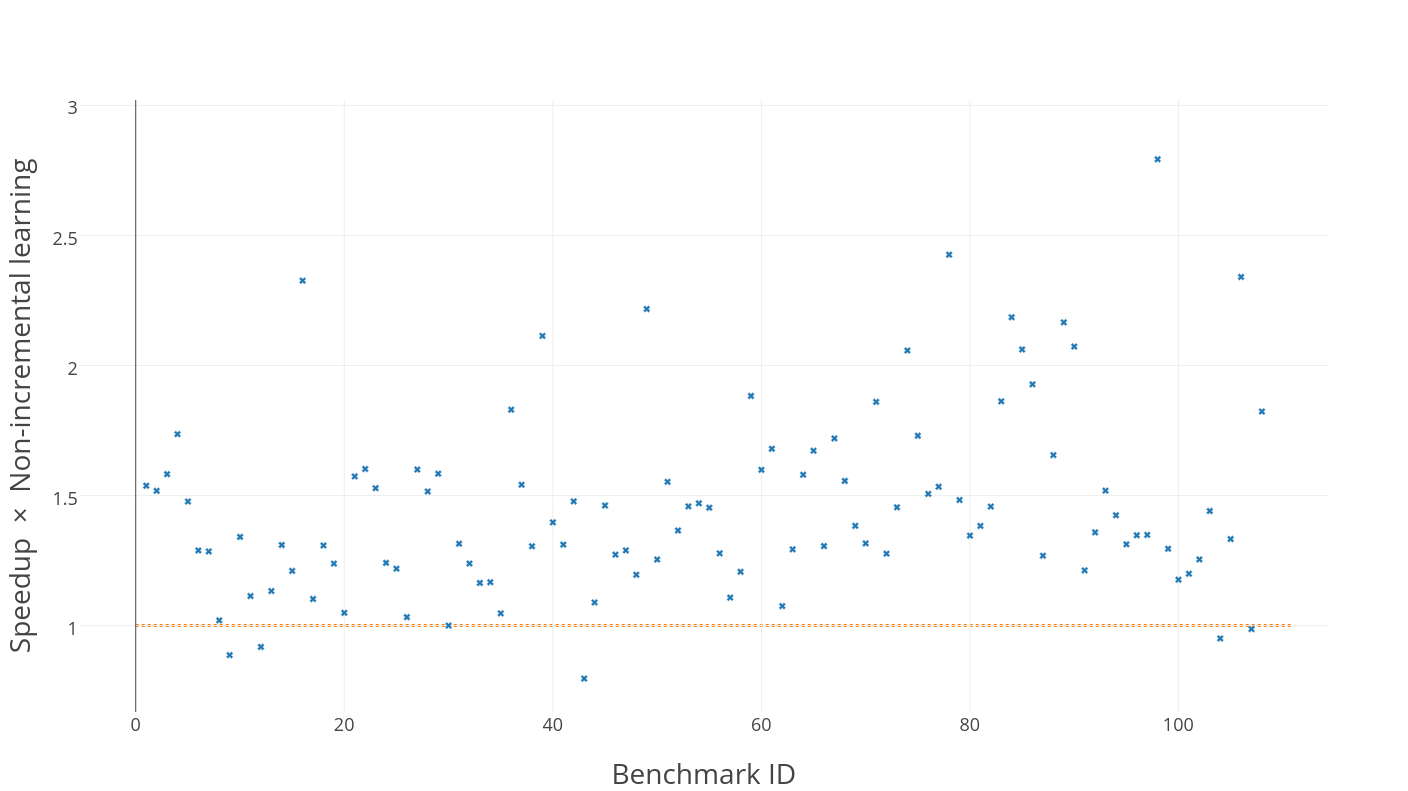
\includegraphics[width=0.99\linewidth]{figures/incremental-learning-performance}
    \caption{Speedups obtained by the incremental synthesis algorithm vs. the non-incremental algorithm when benchmarked
        on 108 real-life FlashFill scenarios (i.e. a subset of our 531 scenarios that requires more than one example).
        Values higher above the $y=1$ line (where the runtimes are equal) are better.}
    \label{fig:interactive:incremental:speedup}
\end{figure}

We evaluate the incremental synthesis algorithm in the context of the FlashFill DSL.
For this case study, we picked all the scenarios which required the user to provide two or more examples to learn a
correct program, from among our collected FlashFill scenarios.
All the data reported in this subsection is obtained by repeating each experiment ten times and averaging the results
after discarding outliers.

\Cref{fig:interactive:incremental:speedup} summarizes the results of our evaluation.
It plots the \emph{speedup} obtained by incremental algorithm over the non-incremental algorithm for each scenario for
the FlashFill DSL.
These were computed by dividing the execution time of the non-incremental algorithm by the execution time of the
incremental algorithm for each scenario.
We observe that almost all the speedup values are greater than one, with the exceptions being extremely short-running
scenarios as mentioned earlier.
Further, the incremental algorithm achieves a geometric mean speedup of 1.42 over the non-incremental algorithm, across
the 108 scenarios considered for the FlashFill DSL.
Despite the relatively small number of learning iterations, our evaluation demonstrates that incrementality yields
significant performance improvements.
